\documentclass{article}
\usepackage[top=1cm, left=1.5cm, right=1.5cm, bottom=1.5cm]{geometry}
\usepackage{graphicx, amsmath, tikz-cd, apacite, amssymb, tcolorbox, wrapfig}
\graphicspath{{./img/}}
\bibliographystyle{apacite}
\setlength{\parindent}{0pt}
\setlength{\parskip}{1em} 
 
\title{Puntos Importantes Ecuaciones Lineales}
\author{Pablo Darío}
\date{09/01/2024}
 
\begin{document}
\maketitle
\section{Combinación Lineal}

El número de entradas en un vector indica la dimensión en $\mathbb{R}$ en la que se encuentra ese vector. El vector cuyas entradas son todas cero se llama \textbf{vector cero} y se denota con 0. Las operaciones de multiplicación escalar y suma vectorial en $\mathbb{R}^n$ se definen entrada por entrada.

Una \textbf{combinación lineal} es la suma de un conjunto de vectores que se multiplican por ciertos escalares, la cual produce otro vector con el mismo número de entradas. $$\mathbf{y} = c_1\mathbf{v_1} + c_2\mathbf{v_2} + \dotsb + c_p\mathbf{v_p}$$

Una ecuación vectorial $$x_1\mathbf{v_1} + x_2\mathbf{v_2} + \dotsb + x_n\mathbf{v_n} = \mathbf{b}$$ tiene el mismo conjunto solución que el sistema lineal cuya matriz aumentada es $$\begin{bmatrix} \mathbf{v_1} & \mathbf{v_2} \dotsb & \mathbf{v_n} & \mathbf{b} \end{bmatrix}$$

En particular \textbf{b} se puede generar por una combinación lineal de $\mathbf{v_1}, \mathbf{v_2},\dots, \mathbf{v_n}$ si y solo si existe una solución al sistema lineal correspondiente a la matriz aumentada anterior.

Si $\mathbf{v_1},\mathbf{v_2},\dots, \mathbf{v_p}$ están en $\mathbb{R}^n$, entonces el conjunto de todas las combinaciones lineales de dicho conjunto se denota como Gen\{$\mathbf{v_1},\mathbf{v_2},\dots, \mathbf{v_p}$\} y se llama \textbf{subconjunto de $\mathbb{R}^n$ generado por $\mathbf{v_1},\mathbf{v_2},\dots, \mathbf{v_p}$}. Es decir Gen\{$\mathbf{v_1},\mathbf{v_2},\dots, \mathbf{v_p}$\} es el conjunto de todos los vectores que se pueden escribir en la forma $$c_1\mathbf{v_1} + c_2\mathbf{v_2} + \dots + c_p\mathbf{v_p}$$ con escalares $c_1,c_2,\dots, c_p$

Preguntar si un vector \textbf{b} está en Gen\{$v_1,v_2,\dots, v_p$\} equivale a preguntar si la ecuación vectorial $$x_1v_1 + x_2v_2 + \dots + x_pv_p = b$$ tiene una solución. La cual se puede reescribir como, 

\begin{equation*}
    x_1 \begin{bmatrix} v_1 \end{bmatrix} 
    +x_2 \begin{bmatrix} v_2 \end{bmatrix}
    + \dotsb + x_p \begin{bmatrix} v_p \end{bmatrix}
    = \begin{bmatrix} b \end{bmatrix}
\end{equation*}

o de manera equivalente, si el sistema lineal con la matriz aumentada $\begin{bmatrix} v_1 & v_2 & \dotsb & v_p & b \end{bmatrix}$ tiene una solución.

Observe que Gen\{$v_1,v_2,\dots, v_p$\} contiene a cada múltiplo escalar de $v_1$ (por ejemplo), ya que $cv_1 = cv_1 + 0v_2 + \dotsb + 0v_p$. Por tanto, el vector cero debe estar en Gen\{$v_1,v_2,\dots, v_p$\}.

\subsection{Descripción Geométrica de Gen\{v\} y de Gen\{u, v\}}

Sea \textbf{v} un vector diferente de cero en $\mathbb{R}^3$. Entonces Gen\{\textbf{v}\} es el conjunto de todos los múltiplos escalares de \textbf{v}, que es el conjunto de puntos sobre la recta en en $\mathbb{R}^3$ que pasa por \textbf{v} y 0. 

Si \textbf{u} y \textbf{v} son vectores diferentes de cero en $\mathbb{R}^3$, y \textbf{v} no es un múltiplo de \textbf{u}, entonces Gen\{\textbf{u},\textbf{v}\} es el plano en $\mathbb{R}^3$ que contiene a \textbf{u}, \textbf{v} y 0. En particular, Gen\{\textbf{u}, \textbf{v}\} contiene la recta en $\mathbb{R}^3$ que pasa por \textbf{u} y 0, y la recta que pasa por \textbf{v} y 0.

\begin{figure}[ht]
    \centerline{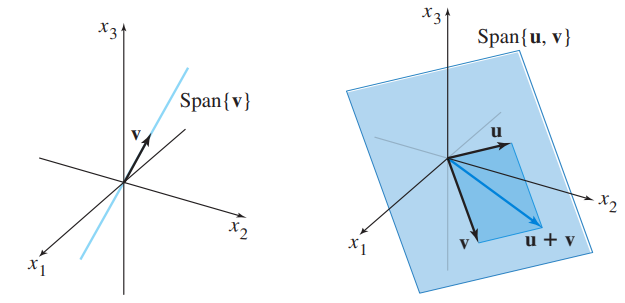
\includegraphics[width=0.6\textwidth]{image11.png}}
    \caption{Gen\{\textbf{$u$}\} y Gen\{\textbf{$u$}, \textbf{$v$}\}}
    \label{}
\end{figure}

\section{Ecuación Matricial}

Si $A$ es una matriz de $m \times n$, con columnas $\mathbf{a_1},\mathbf{a_2},\dots, \mathbf{a_n}$ y si $x$ está en $\mathbb{R}^n$, entonces el producto de $A$ y $x$, denotado como $A\mathbf{x}$, es la combinación lineal de las columnas de $A$ utilizando como pesos las entradas correspondientes en $x$, es decir, $$A\mathbf{x} = \begin{bmatrix}
    \mathbf{a_1},\mathbf{a_2},\dots, \mathbf{a_n} \end{bmatrix} \begin{bmatrix}x_1\\ x_2\\ \vdots \\x_n \end{bmatrix} = x_1\mathbf{a_1} + x_2\mathbf{a_2} + \dotsb + x_n\mathbf{a_n}$$

Si $A$ es una matriz de $m \times n$, con columnas $\mathbf{a_1},\mathbf{a_2},\dots, \mathbf{a_n}$ y si $\mathbf{b}$ está en $\mathbb{R}^n$, la ecuación matricial $$A\mathbf{x} = \mathbf{b}$$ tiene el mismo conjunto solución que la ecuación vectorial $$x_1\mathbf{a_1} + x_2\mathbf{a_2} + \dotsb + x_n\mathbf{a_n} = \mathbf{b}$$ la cual, a la vez tiene el mismo conjunto solución que el sistema de ecuaciones lineales cuya matriz aumentada es $$\begin{bmatrix}\mathbf{a_1}&\mathbf{a_2}& \dotsb & \mathbf{a_n} & \mathbf{b}\end{bmatrix}$$

La ecuación $A\mathbf{x} = \mathbf{b}$ tiene solución si y solo si $\mathbf{b}$ es una combinación lineal de las columas de $A$.

Las columnas de $A$ generan a $\mathbb{R}^m$ significa que cada $\mathbf{b}$ en $\mathbb{R}^m$ es una combinación lineal de las columnas de $A$; cabe recalcar que $c$ hace referencia al número de entradas que tiene cada vector o bien el número de filas de la matriz $A$.

Las columnas de $A$ o un conjunto de vectores $\{\mathbf{v_1}, \mathbf{v_2},..., \mathbf{v_n}\}$ en $\mathbb{R}^m$ genera a $\mathbb{R}^m$ si y solo si la matriz de coeficientes tiene una posición pivote en cada fila, esto porque así la ecuación $A\mathbf{x} = \mathbf{b}$ no puede ser inconsistente o bien no puede tener filas de la siguiente manera: $$\begin{bmatrix}
    0 & 0 & \dotsb & 0 &  \mathbf{b} 
\end{bmatrix}$$

donde \textbf{b} sea un número diferente de 0. 

Si $m>n$ entonces las columnas de $A$ no pueden generar a $\mathbb{R}^m$ debido a que la matriz no puede tener una posición pivote en cada fila; esto significa que hay menos vectores que entradas en cada vector.

\begin{large}
    \textbf{Ejemplo Matriz de $3 \times 2$}
\end{large}

Matriz con 2 vectores en $\mathbb{R}^3$ $$\begin{bmatrix}
    . & *\\
    0 & .\\
    0 & 0
\end{bmatrix}$$

Como observamos la matriz no puede tener una posición pivote en cada fila. Dos vectores en $\mathbb{R}^3$ sería nada más un plano, por lo que un solo plano no puede generar a $\mathbb{R}^3$.

Si $m = n$ entonces la matriz debería tener una posción pivote en cada fila o columna, debido a que es una matriz cuadrada, esto para que las columnas de $A$ generen a $\mathbb{R}^m$.

\begin{large}
    \textbf{Ejemplo Matriz de $3 \times 3$}
\end{large}

$$\begin{bmatrix}
    . & * & *\\
    0 & . & *\\
    0 & 0 & .
\end{bmatrix}$$


Si $m < n$ significa que tenemos más vectores de los necesarios para generar a $\mathbb{R}^m$ por lo que si cada fila tiene una posición pivote si es posible generar a $\mathbb{R}^m$. 

\begin{large}
    \textbf{Ejemplo Matriz de $2 \times 3$}
\end{large}

Para que las columnas de $A$ generen a $\mathbb{R}^m$ en una matriz de $2 \times 3$ necesitamos algunas de las siguientes matrices con pivote en cada fila.

\begin{equation*}
    \begin{bmatrix}
        . & 0 & * \\
        0 & . & *
    \end{bmatrix}, 
    \begin{bmatrix}
        . & * & * \\
        0 & 0 & .
    \end{bmatrix},
    \begin{bmatrix}
        0 & . & * \\
        0 & 0 & .
    \end{bmatrix}
\end{equation*}

En este caso la ecuación $A\mathbf{x} = 0$ tiene infinitas soluciones o bien al menos una variable libre, ya que como se comentó anteriormente tenemos más vectores de los necesarios, por lo que uno o más pueden quedar libres, pero cabe aclarar que no en todos los casos donde $m < n$ se va a generar a $\mathbb{R}^m$, ya que podemos tener el caso donde no todas las filas tengan pivote, ejemplo: 

$$\begin{bmatrix}
    . & * & * \\
    0 & 0 & 0 \\ 
\end{bmatrix}$$

\section{Independencia Lineal}

Se dice que un conjunto indexado de vectores \{$\mathbf{v_1},..., \mathbf{v_p}$\} en $\mathbb{R}^n$ es linealmente independiente si la ecuación vectorial $$x_1\mathbf{v_1} + x_2\mathbf{v_2} + ... + x_p\mathbf{v_p} = 0$$
solo tiene la solución trivial. Se dice que el conjunto \{$\mathbf{v_1},..., \mathbf{v_p}$\} es linealmente dependiente si existen pesos $c_1, ..., c_p$ no todos cero, tales que $$c_1\mathbf{v_1} + c_2\mathbf{v_2} + ... + c_p\mathbf{v_p} = 0$$

Para que la ecuación $A\mathbf{x} = 0$ tengo únicamente la solución trivial, todas las columnas de la matriz $A$ deben tener un pivote.

Un conjunto que solo tiene un vector $\mathbf{v}$ es linealmente independiente si y solo si $\mathbf{v}$ no es el vector cero. Esto se debe a que la ecuación vectorial $x_1\mathbf{v} = 0$ solo tiene la solución trivial cuando $\mathbf{v} \neq 0$. El vector cero es linealmente dependiente porque $x_{1}0=0$
tiene muchas soluciones no triviales.

Un conjunto de dos vectores \{$\mathbf{v_1}, \mathbf{v_2}$\} es linealmente dependiente si al menos uno de los vectores es un múltiplo del otro, esto debido a que son el mismo vector, por lo tanto son dependientes. El conjunto es linealmente independiente si y solo si ninguno de los vectores es un múltiplo del otro.

Un cojunto de dos o más vectores es linealmente dependiente si y solo si al menos uno de los vectores en el conjunto es una combinación lineal de los otros. Esto debido a que uno de los vectores puede ser generado por los demás, es decir ese vector no aporta nada, ya que coexiste en el plano generado por los demás. 

Si $m > n$ pueden ser tanto dependientes como independientes, pero jamás generarán a $\mathbb{R}^m$

\begin{large}
    \textbf{Ejemplo Matriz de $3 \times 2$}
\end{large}

Para que sean independientes: $\mathbb{R}^3$ $$\begin{bmatrix}
    . & *\\
    0 & .\\
    0 & 0
\end{bmatrix}$$

Para que sean dependientes (un vector es múltiplo del otro): $\mathbb{R}^3$ $$\begin{bmatrix}
    . & .\\
    0 & 0\\
    0 & 0
\end{bmatrix}$$

Si $m = n$ pueden ser tanto dependientes como independientes y además si son independientes generan a $\mathbb{R}^m$, esto es cuando todas las filas o todas las columnas de la matriz $A$ tienen pivotes.

\begin{large}
    \textbf{Ejemplo Matriz de $3 \times 3$}
\end{large}

$$\begin{bmatrix}
    . & * & *\\
    0 & . & *\\
    0 & 0 & .
\end{bmatrix}$$

Si $m < n$ el conjunto de vectores siempre van a ser linealmente dependiente, ya que es imposible que todas las columnas tengan pivote, para que generen a $\mathbb{R}^m$ al menos $m$ dos vectores tienen que ser independientes.

\begin{large}
    \textbf{Ejemplo Matriz de $2 \times 3$}
\end{large}

Conjunto de vectores independientes que generan a $\mathbb{R}^m$: $$\begin{bmatrix}
    . & * & *\\
    0 & . & *\\
\end{bmatrix}$$

Conjunto de vectores independientes que \textbf{no} generan a $\mathbb{R}^m$: $$\begin{bmatrix}
    . & * & *\\
    0 & 0 & 0\\
\end{bmatrix}$$

\section{Transformación Lineal}

Una \textbf{transformación} $T$ de $\mathbb{R}^n$ a $\mathbb{R}^m$ es una regla que asigna a cada vector \textbf{x} en $\mathbb{R}^n$ un vector $T$(\textbf{x}) en $\mathbb{R}^m$. El conjunto de $\mathbb{R}^n$ se llama \textbf{dominio} de $T$, y $\mathbb{R}^m$ se llama el \textbf{codominio} de $T$.\\ La notación $T$ : $\mathbb{R}^n \rightarrow \mathbb{R}^m$ indica que el dominio $T$ es $\mathbb{R}^n$ y que el codominio es $\mathbb{R}^m$. Para \textbf{x} en $\mathbb{R}^n$, el vector $T$(\textbf{x}) en $\mathbb{R}^m$ es la \textbf{imagen} de \textbf{x} (bajo la acción o transformación de $T$). El \textbf{conjunto de todas las imágenes} $T$(\textbf{x}) es el \textbf{rango} de $T$.

\begin{figure}[ht]
    \centerline{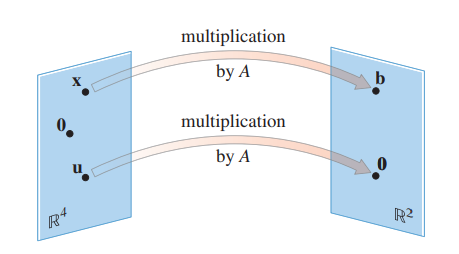
\includegraphics[width=0.4\textwidth]{image16.png}}
    \caption{Transformación Lineal}
  \end{figure}

Para cada \textbf{x} en $\mathbb{R}^n$, $T$(\textbf{x}) se calcula como $A$\textbf{x}, donde $A$ es una matriz de $m \times n$. Para simplificar, algunas veces esta transformación matricial se denota como \textbf{x} $\longmapsto A$\textbf{x}. El dominio de $T$ es $\mathbb{R}^n$ cuando $A$ tiene $n$ columnas y el codominio de $T$ es $\mathbb{R}^m$ cuando las columnas de A tienen $m$ entradas. El rango de $T$ es el conjunto de todas las combinaciones lineales de las columnas de $A$ porque cada imagen $T$(\textbf{x}) es de la forma $A$\textbf{x}.

Para determinar si un vector \textbf{b} está en el rango de una transformación $T$, debemos verificar si \textbf{b} es la imagen vectorial de alguna \textbf{x} en $\mathbb{R}^m$ es decir si $T$(\textbf{x}) = \textbf{b} para alguna \textbf{x}. Esto es otra manera de preguntar si el sistema $A$\textbf{x} = \textbf{b} es consistente.

Los vectores que se van a transformar bajo $T$ de $\mathbb{R}^n$ a $\mathbb{R}^m$ tienen $n$ entradas y los vectores resultantes tienen $m$ entradas.

Sea $T: \mathbb{R}^n \rightarrow \mathbb{R}^m$ una transformación lineal, existe una única matriz $A$ tal que $$T(\mathbf{x}) = A\mathbf{x} \text{ para toda } \textbf{x} \text{ en } \mathbb{R}^n$$
    
$A$ es la matriz de $m \times n$ cuya $j-$ésima columna es el vector $T(\mathbf{e_j})$, donde $\mathbf{e_j}$ es la $j-$ésima columna de la matriz identidad en $\mathbb{R}^n$ $$A = \begin{bmatrix}
        T(\mathbf{e_1}) &\dotsb &T(\mathbf{e_n})
    \end{bmatrix}$$

El término transformación lineal se enfoca sobre una propiedad de un mapeo, mientras que la transformación matricial describe cómo se implementa tal mapeo.

\subsection{Existencia y Unicidad}

Se dice que un mapeo $T: \mathbb{R}^n \rightarrow \mathbb{R}^m$ es \textbf{sobre} $\mathbb{R}^m$ si cada \textbf{b} en $\mathbb{R}^m$ es la imagen de al menos una \textbf{x} en $\mathbb{R}^n$. 

$T$ mapea $\mathbb{R}^n$ sobre $\mathbb{R}^m$ si y solo si las columnas de $A$ generan a $\mathbb{R}^m$.

\begin{figure}[ht]
    \centerline{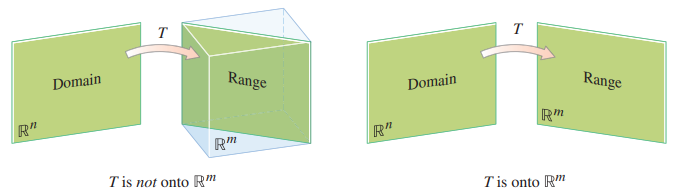
\includegraphics[width=0.8\textwidth]{image22.png}}
    \caption{¿El rango de $T$ es todo $\mathbb{R}^m$?}
\end{figure}
  
Se dice que un mapeo $T: \mathbb{R}^n \rightarrow \mathbb{R}^m$  es \textbf{uno a uno} si cada \textbf{b} en $\mathbb{R}^m$ es la imagen de a lo sumo una \textbf{x} en $\mathbb{R}^n$.

$T$ es uno a uno si, para cada \textbf{b} en $\mathbb{R}^m$, la ecuación $T(\mathbf{x}) = \mathbf{b}$ tiene una única solución o ninguna solución.
  
El mapeo de $T$ no es uno a uno cuando algún \textbf{b} en $\mathbb{R}^m$ es la imagen de más de un vector en $\mathbb{R}^n$. Si no existe tal \textbf{b}, entonces $T$ es uno a uno.
  
\begin{figure}[ht]
    \centerline{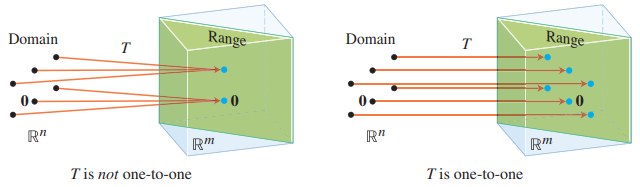
\includegraphics[width=0.8\textwidth]{image23.png}}
    \caption{¿Cada \textbf{b} es la imagen de a lo sumo un vector?}
\end{figure}

$T$ es uno a uno si y solo si la ecuación $T(\mathbf{x}) = 0$ tiene únicamente la solución trivial. 

$T$ es uno a uno si y solo si las columnas de $A$ son linealmente independientes.

\begin{tcolorbox}[colback=red!10!white, colframe=red!70!black, title=Puntos Importantes cuando $m > n$]
    Si $A$ es una matriz de $m \times n$ donde $m > n$ entonces las columnas de $A$ jamás generarán a $\mathbb{R}^m$ debido a que tiene más entradas que vectores y podemos tener una matriz inconsistente donde alguna fila sea de la forma: $$\begin{bmatrix}
        0 & 0 & \dotsb & 0 & \mathbf{b}
    \end{bmatrix}$$,el conjunto de vectores de las columnas de $A$ puede ser independientes o dependiente, recordemos que solo son independientes si todas las columnas de $A$ tienen pivote, esto es que no existe una variable libre o bien que la ecuación $A\mathbf{x} = 0$ solo tenga la solución trivial. El hecho de que sus vectores sean independientes no indica que pueden generar a $\mathbb{R}^m$.
    Una transformación $T: \mathbb{R}^n \rightarrow \mathbb{R}^m$ jamás va ser sobre $\mathbb{R}^m$ debido a que estamos transformando a dimensiones mayores, pero si puede ser uno a uno siempre y cuando las columnas de $A$ sean independientes o que la ecuación $A\mathbf{x} = 0$ solo tenga la solución trivial.\\ 

    \textbf{Sus columnas jamás van a generar a $\mathbb{R}^m$, pero sus columnas pueden ser independientes, su transformación jamás va a ser sobre $\mathbb{R}^m$, pero puede ser uno a uno si sus columnas son independientes, esto es que la ecuación $A\mathbf{x} = 0$ solo tenga la solución trivial.}\\

    \begin{large}
        \textbf{Ejemplo de matrices $3 \times 2$ donde sus columas son independientes y su transformación es uno a uno}
    \end{large}

    \begin{equation*}
        \begin{bmatrix}
            . & *  \\
            0 & * \\
            0 & .
        \end{bmatrix}, 
        \begin{bmatrix}
            . & *  \\
            0 & . \\
            0 & 0
        \end{bmatrix}
    \end{equation*}
    
    \begin{large}
        \textbf{Ejemplo de matrices $3 \times 2$ donde sus columas no son independientes y su transformación no es uno a uno}
    \end{large}

    $$\begin{bmatrix}
        . & *  \\
        0 & 0 \\
        0 & 0
    \end{bmatrix}$$

Cabe recalcar que en ninguno de los 2 ejemplos las columnas de $A$ generan a $\mathbb{R}^m$ y la transformación no es sobre $\mathbb{R}^m$.
\end{tcolorbox}

\begin{tcolorbox}[colback=red!10!white, colframe=red!70!black, title=Puntos Importantes cuando $m$ = $n$ ]
    Si $A$ es una matriz de $m \times n$ donde $m = n$ entonces las columnas de $A$ generan a $\mathbb{R}^m$ si y solo si todas sus filas tienen pivote, si esto ocurre entonces la transformación $T: \mathbb{R}^n \rightarrow \mathbb{R}^m$ es sobre $\mathbb{R}^m$, además significa que cada columna también tiene pivote, por lo que el conjunto de sus columnas son independientes, esto es que la transformación es uno a uno. Esto significa que la ecuación $A\mathbf{x} = 0$ solo tiene la solución trivial.\\

    \begin{large}
        \textbf{Ejemplo de $3 \times 3$ y $2 \times 2$ donde ocurren todos los eventos}

        \begin{equation*}
            \begin{bmatrix}
                . & * & * \\
                0 & . & *\\
                0 & 0 & .
            \end{bmatrix}, 
            \begin{bmatrix}
                . & *  \\
                0 & . 
            \end{bmatrix}
        \end{equation*}

    \end{large}
\end{tcolorbox}

\begin{tcolorbox}[colback=red!10!white, colframe=red!70!black, title=Puntos Importantes cuando $m < n$]
    Si $A$ es una matriz de $m \times n$ donde $m < n$ entonces las columnas de $A$ generan a $\mathbb{R}^m$ si y solo si, cada fila tiene un pivote, esto es si al menos $m$ vectores son independientes; además el conjunto de vectores que conforman las columnas de es linealmente dependiente y si vemos a esta matriz como una matriz transformadora, esta transformación va a ser sobre $\mathbb{R}^m$ si y solo si las columnas de $A$ generan a $\mathbb{R}^m$, además esta transformación $T$ jamás va ser uno a uno porque las columnas de $A$ no son linealmente dependiente. Esta transformación $T: \mathbb{R}^n \rightarrow \mathbb{R}^m$ siempre va a mapear a dimensiones menores. En esta caso la ecuación $A\mathbf{x} = 0$ tiene otras soluciones además de la trivial.\\

    \textbf{Sus columnas jamás van a ser independientes, pero puede generar a $\mathbb{R}^m$. Su transformación jamás va ser uno a uno, pero puede ser sobre $\mathbb{R}^m$ (solo si las columnas de A generan $\mathbb{R}^m$).}\\

    \begin{large}
        \textbf{Ejemplo de matrices $2 \times 3$ que generan a $\mathbb{R}^2$ y su transformación es sobre $\mathbb{R}^2$}
    \end{large}

    \begin{equation*}
        \begin{bmatrix}
            . & 0 & * \\
            0 & . & *
        \end{bmatrix}, 
        \begin{bmatrix}
            . & * & * \\
            0 & 0 & .
        \end{bmatrix},
        \begin{bmatrix}
            0 & . & * \\
            0 & 0 & .
        \end{bmatrix}
    \end{equation*}
    
    \begin{large}
        \textbf{Ejemplo de matrices $2 \times 3$ que no generan a $\mathbb{R}^2$ y su transformación no es sobre $\mathbb{R}^2$}
    \end{large}

    $$\begin{bmatrix}
        . & * & * \\
        0 & 0 & 0 \\ 
    \end{bmatrix}$$

Cabe recalcar que en ninguno de los 2 ejemplos las columnas de $A$ no son independientes y la transformación $T$ no es uno a uno.
\end{tcolorbox}

\end{document}